
%(BEGIN_QUESTION)
% Copyright 2006, Tony R. Kuphaldt, released under the Creative Commons Attribution License (v 1.0)
% This means you may do almost anything with this work of mine, so long as you give me proper credit

An open vessel contains water at 60$^{o}$ F.  A pressure transmitter located at the bottom of the vessel measures the hydrostatic pressure (``head'') generated by the water and outputs a signal corresponding to level.  Suppose that the temperature of this vessel were to increase over time to 110$^{o}$ F due to exposure to very hot outside air (the vessel is located in Death Valley, California during the summer).  Knowing that an increase in water temperature will result in a decrease in density, what will happen to the level transmitter's output as the vessel heats up?  Will the transmitter output increase, decrease, or stay the same?  Why??  Assume that no water enters or exits the vessel during the period of heating from 60$^{o}$ F to 110$^{o}$ F.

\underbar{file i00246}
%(END_QUESTION)





%(BEGIN_ANSWER)

The transmitter output will stay the same.  

\vskip 10pt

If you thought that the transmitter output would decrease due to the water becoming less dense, I recommend you explore the concept of density a little deeper with the following ``thought experiment:''

\begin{itemize}
\item{} Imagine the vessel filled half-way with liquid.
\item{} Imagine that liquid heating up and expanding until it is only {\it half} as dense as it was at the beginning of the experiment.
\item{} Calculate the new hydrostatic pressure with the expanded, less-dense liquid.
\end{itemize}

In a way, this is a ``trick'' question.  As any given mass of water heats up, its volume will increase.  This is what makes it less dense than before: increased volume with the same mass (weight).  Knowing how to calculate hydrostatic pressure from height and specific gravity, you might have approached this problem by assuming the water column height would have stayed the same while its density decreased, resulting in a lesser hydrostatic pressure and decreased transmitter output.  However, this answer is incorrect.

If the water volume expands as a result of a temperature increase, the level inside the vessel {\it must rise}, because it will require a higher vessel level to contain a greater volume of water.  The level will rise by the same percentage that the density decreases, resulting in a cancellation of level increase with density decrease.  As a result, the hydrostatic pressure at any point in the vessel remains constant.

If you have difficulty picturing this effect, consider an exaggerated example to make things simpler.  Suppose that a vessel has been filled to a height of 10 feet with cold liquid:

$$\includegraphics[width=15.5cm]{i00246x01.eps}$$

Now, imagine that same vessel being heated until the liquid expands to exactly {\it twice} its former volume:

$$\includegraphics[width=15.5cm]{i00246x02.eps}$$

The liquid level must double to accommodate twice the volume in the same vessel, assuming a vessel of constant diameter, and its density will be cut in half (twice the volume with the same mass).  Consequently, the two factors of liquid level change and liquid density change cancel each other out to give the exact same hydrostatic pressure as before.  In other words, the transmitter will register the same liquid level as it did when the liquid was cold, and will output the exact same signal, even though the actual vessel level is quite a bit more than it was when cold.  Pretty tricky, huh?

%(END_ANSWER)





%(BEGIN_NOTES)


%INDEX% Measurement, level: hydrostatic pressure

%(END_NOTES)


